\documentclass{article} % For LaTeX2e
\usepackage{iclr2027_conference,times}
\input{math_commands.tex}

\usepackage{hyperref}
\usepackage{url}
\usepackage{graphicx}
\usepackage{booktabs}
\usepackage{multirow}
\usepackage{amsmath}
\usepackage{xcolor}

\title{From {FDG} to {PSMA}: Few-Shot Lesion Segmentation\\
and Representation Transfer in Whole-Body {PET}/{CT}}

% Keep anonymous for workshop submission drafts.
\author{
Anonymous authors\\
Paper under double-blind review
}

\newcommand{\fix}{\marginpar{FIX}}
\newcommand{\new}{\marginpar{NEW}}

% \iclrfinalcopy % Uncomment for camera-ready only.

\begin{document}

\maketitle

\begin{abstract}
Whole-body PET/CT lesion segmentation is highly sensitive to tracer chemistry:
models trained on FDG rarely transfer to PSMA without target labels, yet PSMA
annotations are scarce in many clinical settings. We study this \emph{tracer-shift}
problem under a unified aligned protocol that freezes a shared FDG supervised stage
and varies only the PSMA adaptation budget ($N\in\{50,10,5,0\}$ labeled cases),
plus a high-label PSMA reference ($70\%$) and an FDG held-out test.
Across fifteen method variants spanning classical segmentation, self-supervised
representation learning, promptable PET models, and competition entries, we find that
representation-learning initializations---in particular PET/CT masked autoencoding---
retain higher TEST Dice as PSMA labels vanish, while several strong supervised or
promptable baselines degrade primarily through false negatives on sparse lesions.
We argue that the long-tailed, domain-conditional statistics of clinical findings
should shape both pretraining objectives and evaluation (Dice together with
voxel-level FP/FN), and release code and a mean-metric board for the aligned
protocol.\footnote{Draft for an ICLR workshop track; numbers are live experimental
snapshots and will be frozen for the camera-ready.}
\end{abstract}

\section{Introduction}
\label{sec:intro}

Oncology PET/CT is multimodal and multi-tracer. FDG and PSMA probe overlapping but
statistically different lesion populations: prevalence, SUV patterns, organ
background, and negative-study rates all shift with the tracer
\citep{yixinchen2025hitchhiker}. In practice this yields a representation-learning
problem that is closer to open-world transfer than to i.i.d.\ fine-tuning: abundant
(or at least more available) FDG supervision must support PSMA segmentation when
only a handful of PSMA labels exist.

Recent medical foundation / SSL models promise transferable features
\citep{he2022mae,tang2022self,mae_petct_arxiv}, while strong supervised toolkits such as
nnU-Net remain hard baselines \citep{isensee2021nnu}. Concurrent work on normative
representation learning further emphasizes that clinical findings are rare,
heterogeneous, and imperfectly observed, so objectives and metrics tuned only to
frequent lesions can be misleading \citep{bercea2025normative,bercea2025nova}.

This draft asks a concrete empirical question under matched compute and splits:
\emph{Given the same FDG supervised stage, which initializations and adaptation
recipes remain useful when PSMA labels shrink from 50 to 0 cases?}
Our contributions toward a workshop paper are:
\begin{enumerate}
    \item An \textbf{aligned FDG$\rightarrow$PSMA protocol} with shared FDG training,
    PSMA few-/zero-shot ladders, and TEST reporting of Dice / FP / FN.
    \item A \textbf{multi-method board} covering MIM/nnU-Net, Swin SSL, DpDNet,
    SegAnyPET, PET/CT MAE, retrieval, and AutoPET~V entries.
    \item An analysis linking \textbf{clinical finding statistics} (tracer shift,
    label scarcity, FN-dominated failures) to representation objectives and evaluation.
\end{enumerate}

\section{Aligned experimental protocol}
\label{sec:protocol}

\paragraph{Data.}
We use a stratified PET/CT cohort with tracer-aware roles (PSMA/FDG $\times$
small/large/negative lesion burden) and a fixed 70/10/20 train/val/test split seed.
PSMA few-shot subsets ($N=50,10,5$) are drawn from the PSMA train pool; PSMA
\texttt{fs0} evaluates the shared FDG checkpoint zero-shot on PSMA TEST;
\texttt{fc70\%} uses $70\%$ of PSMA train as a high-label reference; FDG TEST
probes source-domain retention.

\paragraph{Shared FDG stage.}
Every non-retrieval method first trains (or fine-tunes) on the same FDG supervised
split with matched global batch size and a common early-stopping / epoch budget
policy for the board (method-specific defaults are logged). The resulting FDG
checkpoint initializes PSMA adaptation unless the method is training-free.

\paragraph{PSMA adaptation.}
Few-shot fine-tuning uses small labeled PSMA sets with online validation and
TEST evaluation aggregated over nine TEST folds (means reported in the main
text; per-fold grids omitted). Metrics:
\[
\mathrm{Dice}=\frac{2\mathrm{TP}}{2\mathrm{TP}+\mathrm{FP}+\mathrm{FN}},\quad
\mathrm{FP\%}=\frac{\mathrm{FP}}{\mathrm{Neg}},\quad
\mathrm{FN\%}=\frac{\mathrm{FN}}{\mathrm{Pos}},
\]
with Dice computed excluding empty-GT cases and FP/FN as voxel micro-averages.
This decomposition matters clinically: under sparse PSMA disease, mean Dice can
hide near-total miss rates (high FN).

\paragraph{Methods.}
We compare (i) scratch vs.\ pretrained siblings when available;
(ii) PET/CT MAE SSL \citep{mae_petct_arxiv};
(iii) Swin transformer SSL \citep{tang2022self};
(iv) nnU-Net and MIM variants \citep{isensee2021nnu};
(v) DpDNet dual-encoder / scratch \citep{dpdnet2025};
(vi) SegAnyPET pretrained / scratch \citep{seganypet2025};
(vii) prototype retrieval (training-free);
(viii) AutoPET~V competition codebases (BIRTH / YixinChen), scratch and
MultiTalent-initialized rows.

\section{Results}
\label{sec:results}

\begin{figure}[t]
\centering
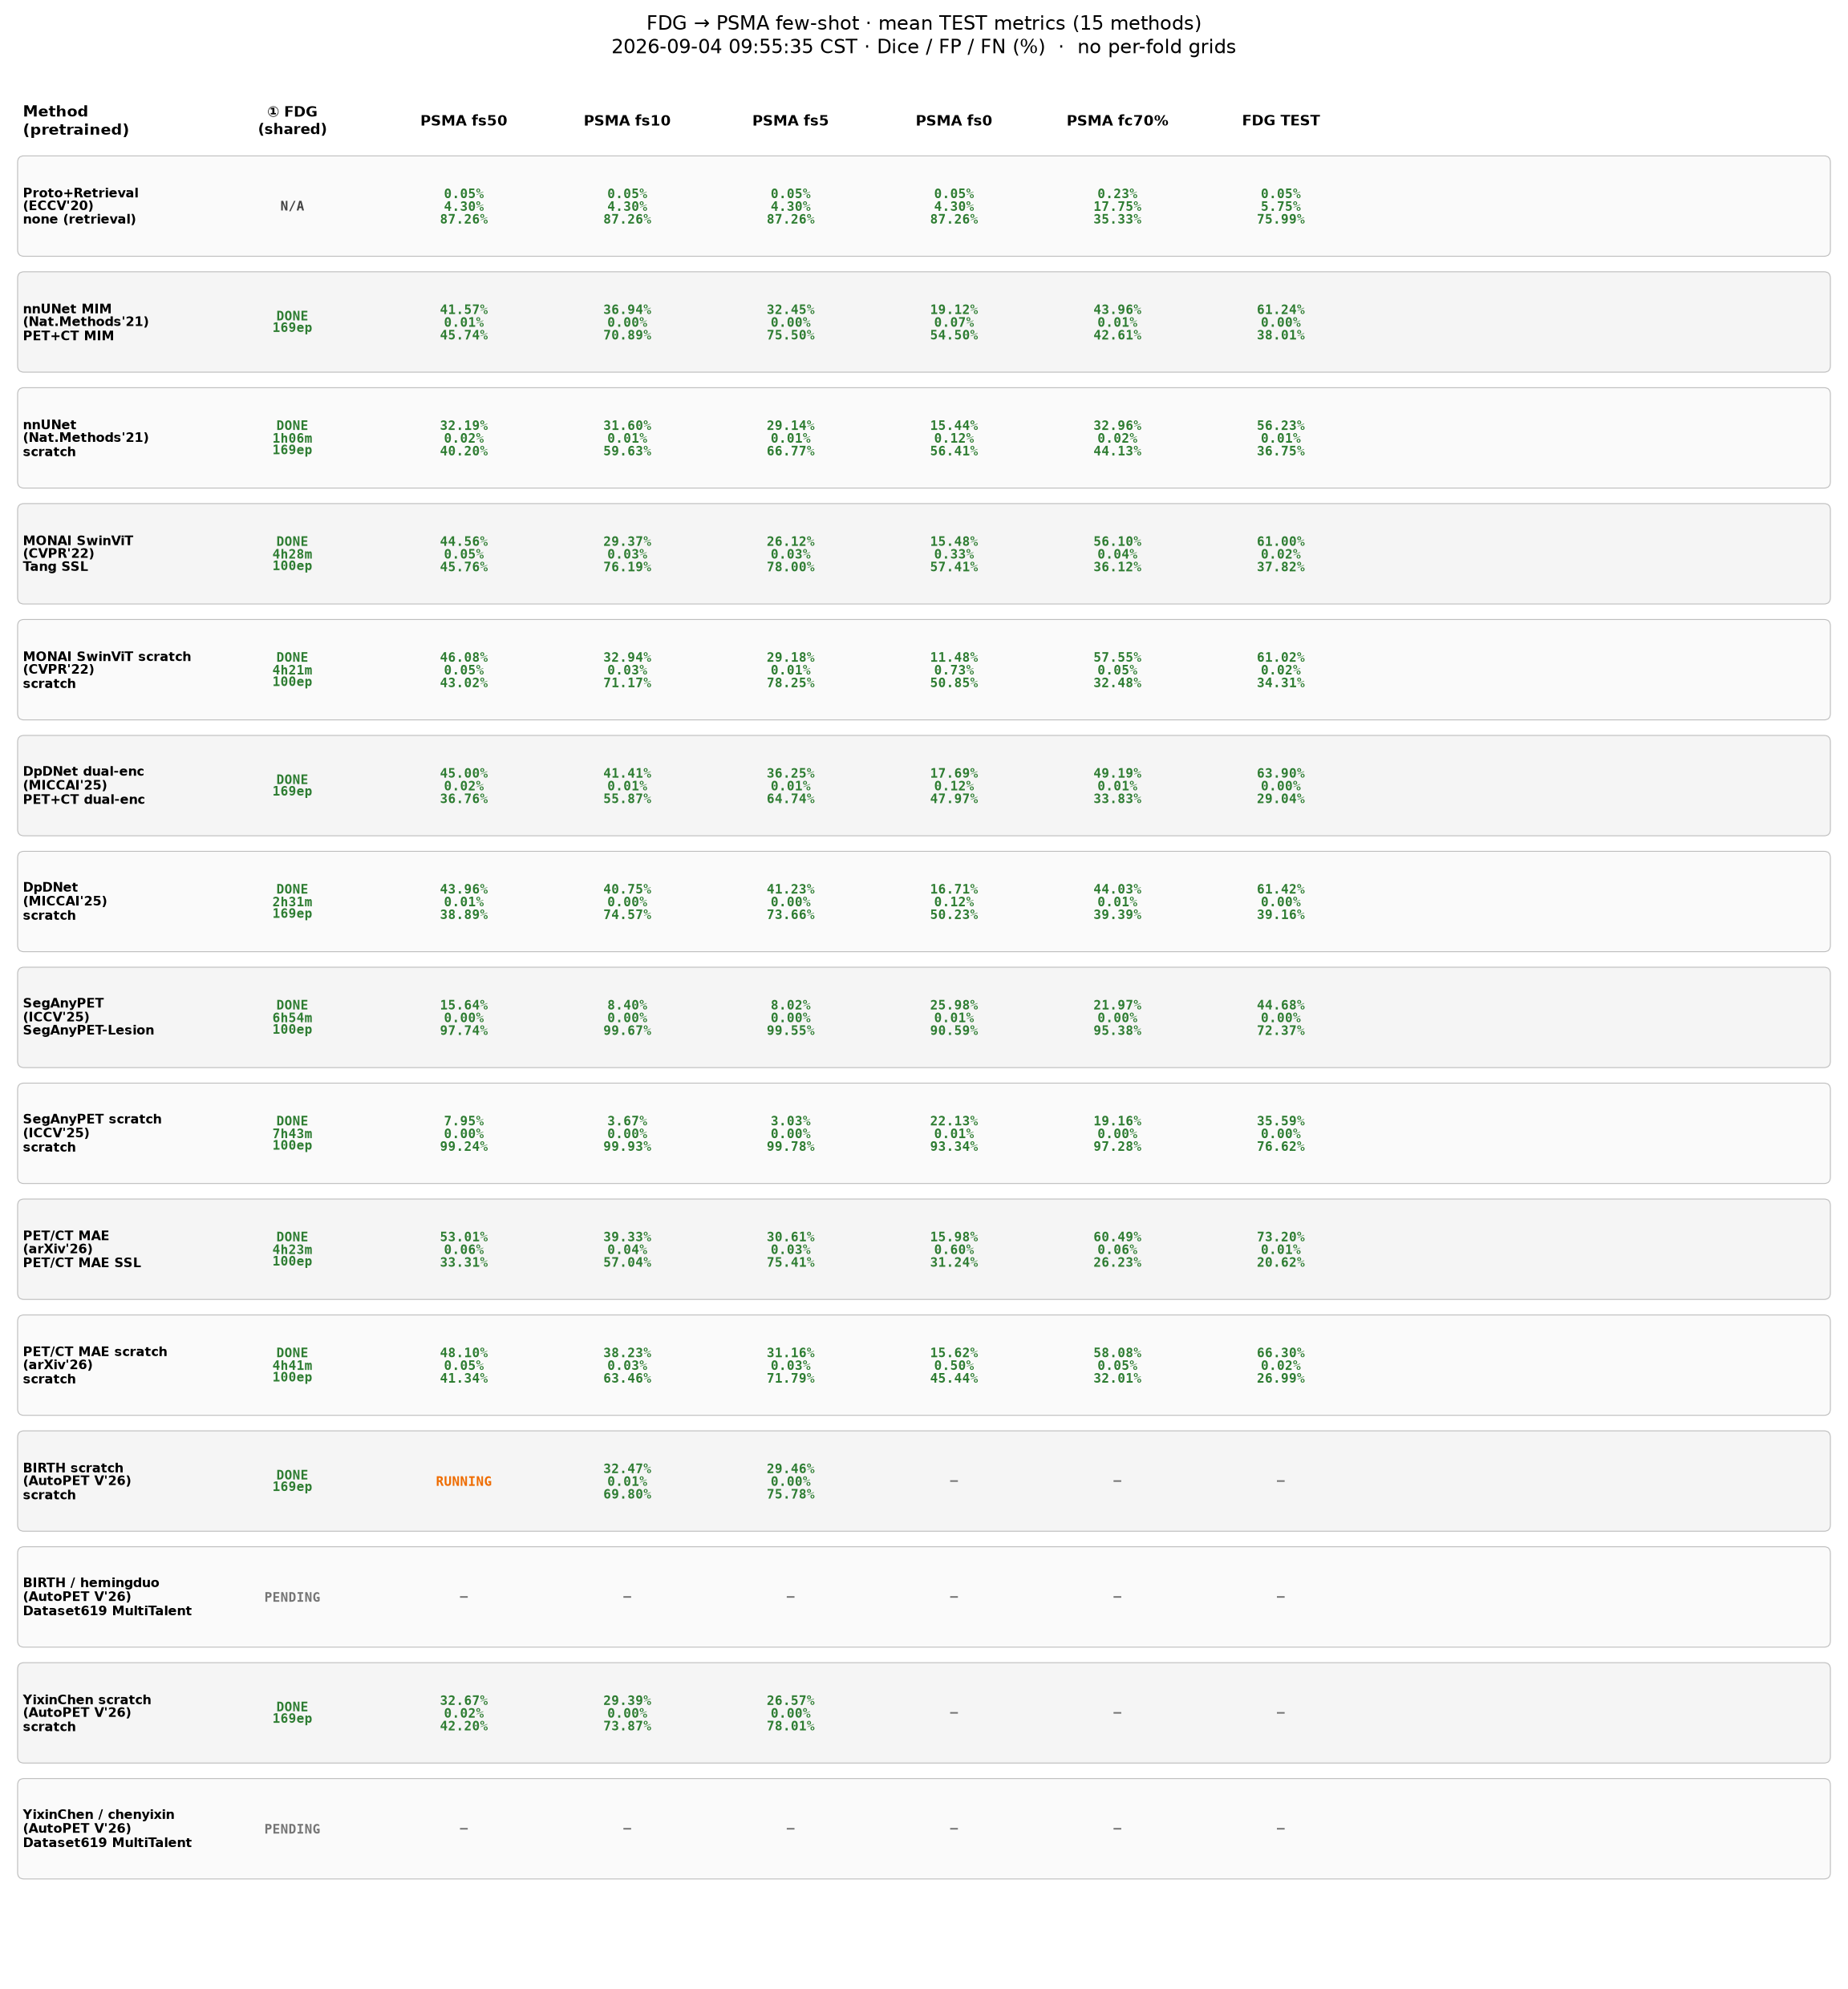
\includegraphics[width=\linewidth]{figures/progress_board.png}
\caption{Mean TEST board for the aligned protocol (Dice / FP / FN).
Nine-fold grids, ETA, and queue footers are omitted. Snapshot timestamp is
embedded in the figure header; incomplete rows remain marked pending/running.}
\label{fig:board}
\end{figure}

\begin{table}[t]
\caption{PSMA/FDG TEST \textbf{Dice (\%)} under the aligned protocol
(higher is better). ``--'' denotes pending/incomplete runs.
Bold marks the best completed entry per column among finished rows.}
\label{tab:dice}
\centering
\scriptsize
\setlength{\tabcolsep}{3.5pt}
\begin{tabular}{llcccccc}
\toprule
Method & Init & fs50 & fs10 & fs5 & fs0 & fc70 & FDG \\
\midrule
Proto+Retrieval & retrieval & 0.0 & 0.0 & 0.0 & 0.0 & 0.2 & 0.0 \\
nnU-Net MIM & MIM & 41.6 & 36.9 & 32.5 & 19.1 & 44.0 & 61.2 \\
nnU-Net & scratch & 32.2 & 31.6 & 29.1 & 15.4 & 33.0 & 56.2 \\
MONAI SwinViT & Tang SSL & 44.6 & 29.4 & 26.1 & 15.5 & 56.1 & 61.0 \\
MONAI SwinViT & scratch & 46.1 & 32.9 & 29.2 & 11.5 & 57.5 & 61.0 \\
DpDNet dual-enc & dual-enc & 45.0 & 41.4 & 36.2 & 17.7 & 49.2 & 63.9 \\
DpDNet & scratch & 44.0 & 40.8 & \textbf{41.2} & 16.7 & 44.0 & 61.4 \\
SegAnyPET & Lesion & 15.6 & 8.4 & 8.0 & \textbf{26.0} & 22.0 & 44.7 \\
SegAnyPET & scratch & 8.0 & 3.7 & 3.0 & 22.1 & 19.2 & 35.6 \\
PET/CT MAE & MAE SSL & \textbf{53.0} & \textbf{39.3} & 30.6 & 16.0 & \textbf{60.5} & \textbf{73.2} \\
PET/CT MAE & scratch & 48.1 & 38.2 & 31.2 & 15.6 & 58.1 & 66.3 \\
BIRTH & scratch & -- & 32.5 & 29.5 & -- & -- & -- \\
BIRTH & MT619 & -- & -- & -- & -- & -- & -- \\
YixinChen & scratch & 32.7 & 29.4 & 26.6 & -- & -- & -- \\
YixinChen & MT619 & -- & -- & -- & -- & -- & -- \\
\bottomrule
\end{tabular}
\end{table}

\paragraph{Representation pretraining helps under scarcity.}
On PSMA \texttt{fs50}, PET/CT MAE with SSL initialization leads completed methods
(53.0 Dice), ahead of its scratch twin (48.1) and of dual-encoder / Swin /
nnU-Net MIM rows (Table~\ref{tab:dice}, Fig.~\ref{fig:board}). The gap persists at
\texttt{fs10}. At \texttt{fs5}, DpDNet scratch is competitive on Dice, but MAE SSL
still pairs stronger FDG TEST retention (73.2), suggesting the SSL features are
not bought by catastrophic forgetting of the source tracer.

\paragraph{Failure modes are statistically asymmetric.}
Board FP rates are typically $\ll 1\%$, while FN often exceeds $30$--$70\%$ as
$N$ decreases---especially for SegAnyPET adaptations that collapse toward
under-segmentation on PSMA few-shot. This matches the clinical prior that
missed sparse lesions dominate error under low prevalence, and argues against
reporting Dice alone.

\paragraph{Zero-shot is not solved.}
PSMA \texttt{fs0} remains low for almost all learned segmentors ($\sim$11--19 Dice),
while SegAnyPET's higher fs0 Dice coexists with very high FN on few-shot columns,
underscoring that training-free / promptable behavior and few-shot fine-tuning
can optimize different operating points.

\section{Discussion: clinical statistics $\leftrightarrow$ objectives}
\label{sec:discussion}

Three statistical facts about findings in this setting should influence
representation learning \citep{bercea2025normative}:
\begin{enumerate}
    \item \textbf{Tracer-conditional normals.} ``Healthy'' and background uptake are
    domain-specific; FDG-pretrained features must be judged by PSMA transfer, not
    only FDG TEST.
    \item \textbf{Long-tailed lesion burden.} Few-shot and empty-GT rates make
    purely discriminative objectives brittle; generative / masked objectives that
    densify anatomical--metabolic structure are a better inductive bias when
    positives are rare.
    \item \textbf{Annotation as a noisy observation model.} Overlap metrics against
    coarse masks can punish conservative segmentors; FP/FN stratification and
    open-world rare-phenotype tests \citep{bercea2025nova} are necessary complements.
\end{enumerate}
We view the aligned board as a stress test of whether a representation was
learned under assumptions compatible with these statistics.

\section{Conclusion}
\label{sec:conclusion}

We presented a draft aligned benchmark for FDG$\rightarrow$PSMA few-shot lesion
segmentation. Early evidence favors PET/CT representation pretraining for
label-scarce PSMA adaptation, while highlighting FN-dominated failures that
Dice alone conceals. Next revisions will freeze incomplete competition rows,
add confidence intervals over folds, and tighten citations for concurrent
PET foundation models.

\subsubsection*{Reproducibility statement}
Code, split JSONs, and the mean-metric board exporter are available at
\url{https://github.com/yeebowang/fdg2psma-fewshot}.
Raw PET/CT volumes and checkpoints are not redistributed here; scripts document
the aligned launchers used to produce Fig.~\ref{fig:board} and Table~\ref{tab:dice}.

\subsubsection*{Ethics statement}
This work uses research PET/CT imaging under existing data-use agreements for
algorithm development. No identifiable patient information is released in the
public repository. Clinical deployment would require prospective validation and
institution-specific governance.

\subsubsection*{AI use statement}
Large language model tools were used to help edit LaTeX wording and repository
documentation. Experimental design, training, evaluation, and numerical results
were produced by the authors' pipelines; the authors verified all reported
metrics against logged board JSON.

\bibliography{references}
\bibliographystyle{iclr2027_conference}

\appendix
\section{Protocol pointers}
Launchers and board ingestion live under \texttt{run/} and
\texttt{scripts/iclr2026\_aligned\_fdg\_fs50\_board.py} in the public repository.
The README figure omits per-fold grids by design; full fold dictionaries remain in
internal board JSON for auditing.

\end{document}
